% ============================================================
%  Python pandas: Beginner to Advanced (scenario based)
%  Compile with:  pdflatex pandas_beginner_to_advanced.tex  (run twice)
%  Based on the official pandas docs: https://pandas.pydata.org/docs/
%  Written for pandas 3.0 (Python 3.11+), most code also works on 2.x
% ============================================================
\documentclass[aspectratio=169,10pt]{beamer}

\usepackage[utf8]{inputenc}
\usepackage[T1]{fontenc}
\usepackage{lmodern}
\usepackage{listings}
\usepackage{xcolor}
\usepackage{tikz}
\usepackage{booktabs}
\usepackage{array}
\usepackage{multicol}

% ---------- Colour palette: calm navy blue + soft light red ----------
\definecolor{navy}{HTML}{1F3A5F}
\definecolor{skyblue}{HTML}{2E6FA7}
\definecolor{paleblue}{HTML}{EAF1F8}
\definecolor{coral}{HTML}{E4767C}
\definecolor{palered}{HTML}{FDEDEE}
\definecolor{deepred}{HTML}{B5424A}
\definecolor{ink}{HTML}{22303F}
\definecolor{codebg}{HTML}{F5F8FB}

% ---------- Theme ----------
\usetheme{Madrid}
\setbeamercolor{palette primary}{bg=navy,fg=white}
\setbeamercolor{palette secondary}{bg=skyblue,fg=white}
\setbeamercolor{palette tertiary}{bg=coral,fg=white}
\setbeamercolor{palette quaternary}{bg=navy,fg=white}
\setbeamercolor{structure}{fg=navy}
\setbeamercolor{normal text}{fg=ink,bg=white}
\setbeamercolor{frametitle}{bg=navy,fg=white}
\setbeamercolor{title}{bg=navy,fg=white}
\setbeamercolor{block title}{bg=skyblue,fg=white}
\setbeamercolor{block body}{bg=paleblue,fg=ink}
\setbeamercolor{block title example}{bg=coral,fg=white}
\setbeamercolor{block body example}{bg=palered,fg=ink}
\setbeamercolor{block title alerted}{bg=deepred,fg=white}
\setbeamercolor{block body alerted}{bg=palered,fg=ink}
\setbeamercolor{item}{fg=coral}
\setbeamercolor{alerted text}{fg=deepred}
\setbeamertemplate{navigation symbols}{}
\setbeamertemplate{itemize items}[circle]
\setbeamerfont{section in toc}{size=\footnotesize}
\setbeamertemplate{section in toc}[sections numbered]
\setbeamerfont{block title}{size=\small,series=\bfseries}
\setbeamerfont{frametitle}{size=\large,series=\bfseries}

% ---------- Code style ----------
\lstdefinestyle{pd}{
  language=Python, basicstyle=\ttfamily\scriptsize, backgroundcolor=\color{codebg},
  keywordstyle=\color{skyblue}\bfseries, commentstyle=\color{deepred}\itshape,
  stringstyle=\color{teal}, showstringspaces=false, frame=single,
  rulecolor=\color{skyblue!40}, columns=fullflexible, keepspaces=true,
  xleftmargin=2pt, xrightmargin=2pt, aboveskip=3pt, belowskip=3pt
}
\lstset{style=pd}

\newcommand{\code}[1]{\texttt{#1}}
\newcommand{\scenario}[1]{\begin{exampleblock}{Real-world scenario}#1\end{exampleblock}}

% ---------- Auto section divider ----------
\AtBeginSection[]{
  \begin{frame}{Where are we?}
    \begin{multicols}{2}
    \tableofcontents[currentsection,hideallsubsections]
    \end{multicols}
  \end{frame}
}

\title[Python pandas]{Python pandas: From Zero to Advanced}
\subtitle{A friendly, scenario-based guide for beginners (age 15+)}
\author{Nafiul Islam}
\institute{BSDS, United International University}
\date{\today}

\begin{document}

\begin{frame}[plain]
  \titlepage
\end{frame}

% ============================================================
\begin{frame}{What you will learn}
  \begin{multicols}{2}
  \tableofcontents[hideallsubsections]
  \end{multicols}
  \begin{block}{How to use these slides}
    Every tool comes with a \textbf{real-life story}, a \textbf{short code example}, and a
    \textbf{``when to use it''} tip. Type the code yourself. That is the fastest way to learn.
  \end{block}
\end{frame}

\begin{frame}{Our running story: ``Sunny Mart'' online shop}
  Imagine you just got a job at \textbf{Sunny Mart}, a small online shop. Your boss gives you
  an Excel/CSV file with every order. You must answer questions like:
  \begin{itemize}
    \item Which city buys the most?
    \item Which product earns the most money?
    \item Are sales growing month by month?
    \item Who are our best customers?
  \end{itemize}
  \vspace{1mm}
  \begin{tabular}{@{}llllrrl@{}}
    \toprule
    \textbf{order\_id} & \textbf{customer} & \textbf{city} & \textbf{product} & \textbf{qty} & \textbf{price} & \textbf{date}\\
    \midrule
    1001 & Rafi & Dhaka & Headphones & 2 & 25 & 2026-01-05\\
    1002 & Mim & Chattogram & Phone case & 1 & 8 & 2026-01-07\\
    1003 & Sara & Dhaka & Keyboard & 1 & 30 & 2026-01-09\\
    \bottomrule
  \end{tabular}
\end{frame}

% ============================================================
\section{Meet pandas}

\begin{frame}{What is pandas?}
  \begin{columns}[T]
    \column{0.55\textwidth}
    \textbf{pandas} is a Python library for working with \alert{tables of data}
    (rows and columns), just like Excel, but with superpowers.
    \begin{itemize}
      \item Open files (CSV, Excel, JSON, databases)
      \item Clean messy data
      \item Filter, sort, group, and summarize
      \item Join tables together
      \item Handle dates and time
    \end{itemize}
    \column{0.43\textwidth}
    \scenario{Your CSV has 500{,}000 orders. Excel freezes. pandas handles it in seconds
    and you can repeat the same steps tomorrow with one click.}
  \end{columns}
  \vspace{1mm}
  \begin{alertblock}{Name fun fact}
    ``pandas'' comes from \emph{panel data}, not the animal!
  \end{alertblock}
\end{frame}

\begin{frame}[fragile]{Install and import}
\begin{lstlisting}
# In your terminal (needs Python 3.11+ for pandas 3.0)
pip install pandas
pip install pyarrow openpyxl      # optional helpers: fast files + Excel
\end{lstlisting}
\begin{lstlisting}
import pandas as pd               # everyone writes "pd"
import numpy as np                # pandas' partner for maths

print(pd.__version__)             # check your version
\end{lstlisting}
  \begin{block}{Tip}
    Use \textbf{Jupyter Notebook} or \textbf{Google Colab}. You see the table right below
    your code, which is perfect for learning.
  \end{block}
\end{frame}

\begin{frame}{The two main objects}
  \begin{columns}[T]
    \column{0.48\textwidth}
    \begin{block}{Series = one column}
      A list of values \textbf{with labels} (the index).\\[1mm]
      Like one column in Excel.
    \end{block}
    \column{0.48\textwidth}
    \begin{block}{DataFrame = whole table}
      Many Series sharing one index.\\[1mm]
      Like an entire Excel sheet.
    \end{block}
  \end{columns}
  \vspace{2mm}
  \begin{center}
  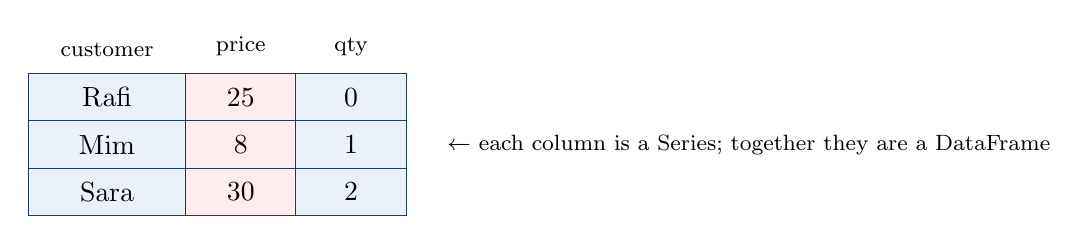
\begin{tikzpicture}[x=1cm,y=1cm]
    \foreach \i/\n/\p in {0/Rafi/25,1/Mim/8,2/Sara/30}{
      \node[draw=navy,fill=paleblue,minimum width=2cm,minimum height=0.6cm] at (0,-\i*0.6) {\n};
      \node[draw=navy,fill=palered,minimum width=1.4cm,minimum height=0.6cm] at (1.7,-\i*0.6) {\p};
      \node[draw=navy,fill=paleblue,minimum width=1.4cm,minimum height=0.6cm] at (3.1,-\i*0.6) {\i};
    }
    \node[above] at (0,0.4) {\footnotesize customer};
    \node[above] at (1.7,0.4) {\footnotesize price};
    \node[above] at (3.1,0.4) {\footnotesize qty};
    \node[right] at (4.2,-0.6) {\footnotesize $\leftarrow$ each column is a Series; together they are a DataFrame};
  \end{tikzpicture}
  \end{center}
\end{frame}

\begin{frame}[fragile]{Series: one column of data}
\begin{lstlisting}
temps = pd.Series([31, 33, 29, 35], index=["Mon", "Tue", "Wed", "Thu"])
print(temps)
# Mon    31
# Tue    33 ...

temps["Tue"]          # 33   -> get by label
temps.mean()          # 32.0 -> quick maths
temps + 2             # adds 2 to EVERY value (no loop needed!)
temps[temps > 30]     # only days hotter than 30
\end{lstlisting}
  \scenario{Your weather app stores daily temperatures. A Series lets you find hot days,
  compute averages, and fix all values at once.}
  \begin{block}{Key idea: vectorization}
    Operations apply to \alert{all values together}. No \code{for} loops needed.
  \end{block}
\end{frame}

\begin{frame}[fragile]{Create a DataFrame}
\begin{lstlisting}
orders = pd.DataFrame({
    "order_id": [1001, 1002, 1003, 1004],
    "customer": ["Rafi", "Mim", "Sara", "Rafi"],
    "city":     ["Dhaka", "Chattogram", "Dhaka", "Sylhet"],
    "product":  ["Headphones", "Phone case", "Keyboard", "Mouse"],
    "qty":      [2, 1, 1, 3],
    "price":    [25.0, 8.0, 30.0, 12.5],
})
orders
\end{lstlisting}
\textbf{Other ways to build one:}
\begin{lstlisting}
pd.DataFrame([{"a": 1, "b": 2}, {"a": 3, "b": 4}])      # list of dicts (API data)
pd.DataFrame(np.random.rand(3, 2), columns=["x", "y"])  # from a NumPy array
\end{lstlisting}
\end{frame}

\begin{frame}[fragile]{Reading files: \texttt{read\_csv} and options}
\begin{lstlisting}
df = pd.read_csv("sunnymart_orders.csv")

df = pd.read_csv(
    "sunnymart_orders.csv",
    usecols=["order_id", "city", "qty", "price", "date"],  # load only needed columns
    parse_dates=["date"],          # turn text into real dates
    dtype={"order_id": "int32"},   # choose smaller types
    na_values=["N/A", "-", ""],    # words that mean "missing"
    nrows=1000,                    # peek at only the first 1000 rows
)
\end{lstlisting}
  \scenario{Your boss sends a 2 GB file. Use \code{usecols} and \code{nrows} first to test
  your code quickly without waiting minutes.}
\end{frame}

\begin{frame}[fragile]{Reading and writing other formats}
\begin{lstlisting}
pd.read_excel("report.xlsx", sheet_name="January")    # needs openpyxl
pd.read_json("api_data.json")
pd.read_parquet("big_data.parquet")                   # fast, compressed (pyarrow)
pd.read_sql("SELECT * FROM orders", connection)       # from a database

# Saving results
df.to_csv("clean_orders.csv", index=False)            # index=False avoids extra column
df.to_excel("summary.xlsx", index=False)
df.to_parquet("clean_orders.parquet")
\end{lstlisting}
  \begin{block}{When to use what}
    \textbf{CSV}: simple, shareable. \textbf{Excel}: for managers. \textbf{Parquet}: big data,
    fast and small. \textbf{SQL}: data lives in a company database.
  \end{block}
\end{frame}

\begin{frame}[fragile]{Your first look at any dataset}
\begin{lstlisting}
df.head()          # first 5 rows
df.tail(3)         # last 3 rows
df.shape           # (rows, columns), e.g. (1200, 7)
df.columns         # column names
df.dtypes          # data type of each column
df.info()          # types + how many values are NOT missing
df.describe()      # count, mean, min, max... for number columns
df.sample(5)       # 5 random rows (great for spotting weird data)
\end{lstlisting}
  \scenario{A new CSV lands in your inbox. Before any analysis, run \code{head}, \code{info},
  and \code{describe}. Think of it as a doctor's check-up for data.}
\end{frame}

\begin{frame}[fragile]{The index: row labels}
\begin{lstlisting}
df = df.set_index("order_id")      # use order_id as the row label
df.loc[1002]                       # find an order directly by its id
df = df.reset_index()              # turn the index back into a normal column
\end{lstlisting}
  \begin{itemize}
    \item The index is like a \textbf{roll number}: it identifies each row.
    \item Default index is \code{0, 1, 2, \dots}
    \item Good index choices: IDs, dates. Bad choices: columns with repeated values.
  \end{itemize}
  \begin{alertblock}{Remember}
    After filtering or sorting, index labels do \alert{not} renumber. Use
    \code{reset\_index(drop=True)} for a fresh 0, 1, 2\dots
  \end{alertblock}
\end{frame}

% ============================================================
\section{Selecting data}

\begin{frame}[fragile]{Selecting columns}
\begin{lstlisting}
df["city"]                    # ONE column  -> a Series
df[["city", "price"]]         # SEVERAL columns -> a DataFrame (note double brackets)
df.city                       # works, but breaks if the name has spaces. Avoid.
\end{lstlisting}
  \scenario{The marketing team only needs customer names and cities. Select just those two
  columns and send them a small file.}
  \begin{alertblock}{Common mistake}
    \code{df["city","price"]} gives a \textbf{KeyError}. Use a \emph{list} inside:
    \code{df[["city","price"]]}.
  \end{alertblock}
\end{frame}

\begin{frame}{\texttt{loc} vs \texttt{iloc}: the most important choice}
  \begin{center}
  \renewcommand{\arraystretch}{1.3}
  \begin{tabular}{p{2.2cm}p{4.2cm}p{4.8cm}}
    \toprule
     & \textbf{loc} & \textbf{iloc}\\
    \midrule
    Selects by & \textbf{L}abels (names) & \textbf{I}nteger positions\\
    Slice end & \alert{Included} & Excluded (like Python lists)\\
    Example & \code{df.loc[2, "city"]} & \code{df.iloc[2, 1]}\\
    Best for & Readable code, filtering + assigning & ``Give me the first 10 rows''\\
    \bottomrule
  \end{tabular}
  \end{center}
  \vspace{2mm}
  \scenario{\textbf{loc} = ``find the student named Rafi''. \textbf{iloc} = ``find the
  student sitting in seat number 3''.}
\end{frame}

\begin{frame}[fragile]{\texttt{loc} and \texttt{iloc} in action}
\begin{lstlisting}
df.loc[0]                          # row with label 0
df.loc[0:2, ["customer", "city"]]  # rows 0,1,2 (end INCLUDED), two columns
df.loc[df["qty"] > 1, "product"]   # rows where qty>1, only product column

df.iloc[0]                         # first row
df.iloc[0:2, 0:3]                  # rows 0,1 and columns 0,1,2 (end EXCLUDED)
df.iloc[-1]                        # last row
df.iloc[:, 1]                      # all rows, 2nd column
\end{lstlisting}
  \begin{block}{Rule of thumb}
    Prefer \code{loc} with column \emph{names}. Column positions change; names are stable and
    make your code easy to read.
  \end{block}
\end{frame}

\begin{frame}[fragile]{Filtering rows with conditions}
\begin{lstlisting}
df[df["city"] == "Dhaka"]         # orders from Dhaka
df[df["price"] > 20]              # expensive items
df[df["qty"] >= 3]                # bulk orders
df[df["customer"] != "Rafi"]      # everyone except Rafi
\end{lstlisting}
  \textbf{How it works:} \code{df["price"] > 20} makes a list of True/False (a \emph{mask}).
  pandas keeps only the rows marked True.
  \scenario{Support asks: ``Show me every order above \$20 from Dhaka.'' Two conditions, one
  filter. See the next slide.}
\end{frame}

\begin{frame}[fragile]{Combining conditions: \&, |, \~{}}
\begin{lstlisting}
# AND  ->  &      (always wrap each condition in parentheses!)
df[(df["city"] == "Dhaka") & (df["price"] > 20)]

# OR   ->  |
df[(df["city"] == "Dhaka") | (df["city"] == "Sylhet")]

# NOT  ->  ~
df[~(df["city"] == "Dhaka")]
\end{lstlisting}
  \begin{alertblock}{Do NOT use Python's and / or / not here}
    They raise \textbf{ValueError: truth value of a Series is ambiguous}. Use \code{\&},
    \code{|}, \code{\~{}} and put parentheses around each condition.
  \end{alertblock}
\end{frame}

\begin{frame}[fragile]{Handy filters: isin, between, str.contains}
\begin{lstlisting}
df[df["city"].isin(["Dhaka", "Sylhet"])]          # value is in a list
df[df["price"].between(10, 30)]                   # 10 <= price <= 30
df[df["product"].str.contains("phone", case=False)]   # text search
df[df["customer"].str.startswith("R")]            # names starting with R
df[df["date"].notna()]                            # rows where date exists
\end{lstlisting}
  \scenario{A summer sale only applies to Dhaka and Sylhet (\code{isin}), items priced
  between \$10 and \$30 (\code{between}), and products with ``phone'' in the name
  (\code{str.contains}).}
  \begin{block}{When to use}
    \code{isin} replaces many \code{|} conditions. \code{between} replaces \code{>= \& <=}.
  \end{block}
\end{frame}

\begin{frame}[fragile]{\texttt{query()}: filters that read like English}
\begin{lstlisting}
df.query("city == 'Dhaka' and price > 20")

min_price = 20
df.query("price > @min_price")                    # use Python variables with @
df.query("city in ['Dhaka', 'Sylhet'] and qty >= 2")
\end{lstlisting}
  \begin{itemize}
    \item Shorter and cleaner when you have many conditions.
    \item Great inside \alert{method chains} (we will meet them later).
    \item Column names with spaces need backticks: \code{`order date`}.
  \end{itemize}
\end{frame}

\begin{frame}[fragile]{Changing values safely}
\begin{lstlisting}
# Change one cell
df.loc[0, "price"] = 27.0

# Change many cells that match a condition
df.loc[df["city"] == "Dhaka", "delivery_fee"] = 2.0
df.loc[df["city"] != "Dhaka", "delivery_fee"] = 5.0
\end{lstlisting}
  \begin{alertblock}{Never use ``chained assignment''}
    \code{df[df["city"]=="Dhaka"]["price"] = 0} does \textbf{not} change \code{df}.
    pandas 3.0 uses \textbf{Copy-on-Write}: the first part creates a copy, so you edit
    the copy only. Always write \code{df.loc[mask, "column"] = value}.
  \end{alertblock}
\end{frame}

\begin{frame}{Selecting: which tool should I use?}
  \renewcommand{\arraystretch}{1.25}
  \begin{center}
  \small
  \begin{tabular}{p{5.3cm}p{5.8cm}}
    \toprule
    \textbf{I want to\dots} & \textbf{Use}\\
    \midrule
    One or more columns & \code{df["a"]}, \code{df[["a","b"]]}\\
    Row/column by name & \code{df.loc[...]}\\
    Row/column by position & \code{df.iloc[...]}\\
    Rows matching a condition & \code{df[mask]} or \code{df.query()}\\
    Value in a list of choices & \code{.isin([...])}\\
    Value within a range & \code{.between(a, b)}\\
    Text contains a word & \code{.str.contains("word")}\\
    Change values by condition & \code{df.loc[mask, "col"] = value}\\
    \bottomrule
  \end{tabular}
  \end{center}
\end{frame}

% ============================================================
\section{Cleaning messy data}

\begin{frame}[fragile]{Step 1: find missing values}
\begin{lstlisting}
df.isna()                      # True where a value is missing (NaN)
df.isna().sum()                # count of missing values per column
df.isna().mean() * 100         # percent missing per column
df[df["city"].isna()]          # see the rows with missing city
\end{lstlisting}
  \scenario{Customers sometimes skip the ``city'' box when ordering. Before delivering
  anything, count how many orders have no city.}
  \begin{block}{Why it matters}
    Missing values silently break averages, sorting, and joins. Always check them first.
  \end{block}
\end{frame}

\begin{frame}[fragile]{Step 2: drop or fill?}
\begin{lstlisting}
df.dropna()                          # remove rows with ANY missing value
df.dropna(subset=["city", "price"])  # only care about these columns
df.dropna(thresh=5)                  # keep rows with at least 5 real values

df["city"] = df["city"].fillna("Unknown")          # fill with a label
df["price"] = df["price"].fillna(df["price"].median())  # fill with typical value
df["stock"] = df["stock"].ffill()                  # copy the previous value down
\end{lstlisting}
  \begin{columns}[T]
    \column{0.48\textwidth}
    \begin{block}{Drop when\dots}
      Few rows are missing, or the key info (like price) is missing.
    \end{block}
    \column{0.48\textwidth}
    \begin{block}{Fill when\dots}
      You can make a smart guess: median price, ``Unknown'', or the last known value.
    \end{block}
  \end{columns}
\end{frame}

\begin{frame}[fragile]{Duplicates}
\begin{lstlisting}
df.duplicated().sum()                 # how many fully repeated rows?
df[df.duplicated(keep=False)]         # look at ALL copies before deleting
df = df.drop_duplicates()             # remove exact repeats
df = df.drop_duplicates(subset="order_id", keep="last")   # keep the latest per id
\end{lstlisting}
  \scenario{The payment system sent order \#1005 twice because of a network glitch. If you
  don't remove it, revenue is counted double!}
\end{frame}

\begin{frame}[fragile]{Fixing data types}
\begin{lstlisting}
df["price"] = pd.to_numeric(df["price"], errors="coerce")   # bad text -> NaN
df["date"]  = pd.to_datetime(df["date"])                    # text -> real dates
df["qty"]   = df["qty"].astype("int32")                     # smaller integer
df["city"]  = df["city"].astype("category")                 # repeated labels
\end{lstlisting}
  \scenario{The price column contains ``\$25'', ``twenty'', and ``30''. Because of the text,
  pandas can't add them. \code{to\_numeric(errors="coerce")} converts what it can and marks
  the rest as missing so you can decide what to do.}
  \begin{block}{Why types matter}
    Dates as real dates allow month/year tricks. Numbers as numbers allow maths.
  \end{block}
\end{frame}

\begin{frame}[fragile]{Renaming and dropping}
\begin{lstlisting}
df = df.rename(columns={"cust": "customer", "prc": "price"})

# Clean ALL column names at once: lowercase, no spaces
df.columns = df.columns.str.strip().str.lower().str.replace(" ", "_")

df = df.drop(columns=["notes", "temp_id"])      # remove columns
df = df.drop(index=[0, 5])                      # remove rows by label
\end{lstlisting}
  \scenario{Two teammates exported files: one has ``Order Date'', the other ``order\_date''.
  Cleaning names to lowercase with underscores makes merging easy.}
\end{frame}

\begin{frame}[fragile]{Cleaning text with \texttt{.str}}
\begin{lstlisting}
s = df["customer"]
s.str.strip()                    # remove extra spaces: "  Rafi " -> "Rafi"
s.str.lower()                    # "RAFI" -> "rafi"
s.str.title()                    # "rafi khan" -> "Rafi Khan"
s.str.replace("-", " ")          # replace pieces of text
s.str.split(" ", expand=True)    # split into separate columns
s.str.len()                      # length of each text
s.str.extract(r"(\d+)")          # pull out digits with a regex
\end{lstlisting}
  \scenario{Cities were typed as ``dhaka'', ``DHAKA'', and `` Dhaka ''. Without cleaning,
  pandas counts them as 3 different cities! Use \code{.str.strip().str.title()}.}
\end{frame}

\begin{frame}[fragile]{Replacing and mapping values}
\begin{lstlisting}
df["city"] = df["city"].replace({"Dacca": "Dhaka", "Ctg": "Chattogram"})

status_map = {0: "Pending", 1: "Shipped", 2: "Delivered"}
df["status_text"] = df["status"].map(status_map)
\end{lstlisting}
  \begin{block}{replace vs map}
    \code{replace}: fix \emph{some} values, leave the rest. \\
    \code{map}: translate \emph{every} value; anything not in the dictionary becomes NaN.
  \end{block}
  \scenario{The database stores status as codes 0/1/2. Your report needs readable words.
  Use \code{map}.}
\end{frame}

\begin{frame}[fragile]{Spotting outliers}
\begin{lstlisting}
df["price"].describe()                         # min/max look strange?
q1, q3 = df["price"].quantile([0.25, 0.75])
iqr = q3 - q1
low, high = q1 - 1.5 * iqr, q3 + 1.5 * iqr    # the "IQR rule"

df[(df["price"] < low) | (df["price"] > high)] # inspect the outliers
df["price"] = df["price"].clip(lower=low, upper=high)   # cap extreme values
\end{lstlisting}
  \scenario{One order says price = 25000 because someone typed two extra zeros. It makes the
  average price look crazy. Find it, then fix it or cap it.}
\end{frame}

\begin{frame}{Cleaning checklist}
  \begin{enumerate}
    \item \textbf{Look}: \code{head, info, describe}
    \item \textbf{Fix names}: lowercase, no spaces
    \item \textbf{Fix types}: numbers, dates, categories
    \item \textbf{Missing values}: \code{isna().sum()}, then drop or fill
    \item \textbf{Duplicates}: \code{duplicated()}
    \item \textbf{Text}: strip, lower/title, replace typos
    \item \textbf{Outliers}: \code{describe}, IQR, \code{clip}
    \item \textbf{Save} the clean file with \code{to\_csv}
  \end{enumerate}
  \begin{block}{Real-life fact}
    Data scientists spend most of their time cleaning data. Learn this section well!
  \end{block}
\end{frame}

% ============================================================
\section{Creating and transforming columns}

\begin{frame}[fragile]{New columns from old columns}
\begin{lstlisting}
df["total"] = df["qty"] * df["price"]
df["price_with_tax"] = df["price"] * 1.15
df["full_name"] = df["first"] + " " + df["last"]
df["month"] = df["date"].dt.month
df["is_big_order"] = df["total"] > 100          # True/False column
\end{lstlisting}
  \scenario{Revenue for each order = quantity times price. One line creates it for all
  500{,}000 rows at once.}
\end{frame}

\begin{frame}[fragile]{\texttt{assign} and \texttt{pd.col} (new in pandas 3.0)}
\begin{lstlisting}
# assign() returns a NEW DataFrame, so it fits in chains
df2 = df.assign(total=df["qty"] * df["price"])

# pandas 3.0: pd.col("name") refers to a column without repeating "df"
df2 = df.assign(
    total=pd.col("qty") * pd.col("price"),
    tax=pd.col("qty") * pd.col("price") * 0.15,
)
\end{lstlisting}
  \begin{block}{When to use}
    Use \code{df["new"] = ...} for quick work. Use \code{assign} when you build step-by-step
    pipelines and don't want to modify the original table.
  \end{block}
\end{frame}

\begin{frame}[fragile]{If-else logic: \texttt{np.where} and \texttt{np.select}}
\begin{lstlisting}
# One condition (like Excel IF)
df["size"] = np.where(df["total"] >= 100, "Big", "Small")

# Many conditions (like IFS)
conditions = [df["total"] >= 200, df["total"] >= 100, df["total"] >= 50]
labels     = ["Premium", "Big", "Medium"]
df["tier"] = np.select(conditions, labels, default="Small")
\end{lstlisting}
  \scenario{Free delivery for orders of \$100+. Loyalty tiers for Premium, Big, Medium, and
  Small orders. \code{np.where} handles two outcomes; \code{np.select} handles many.}
  \begin{block}{Also useful}
    \code{s.where(cond, other)} keeps values where True, replaces others. \code{s.mask(cond, other)} does the opposite.
  \end{block}
\end{frame}

\begin{frame}[fragile]{\texttt{map} and \texttt{apply}: custom logic}
\begin{lstlisting}
# map: Series, one value at a time
df["city_short"] = df["city"].map({"Dhaka": "DHK", "Chattogram": "CTG"})

# apply on a Series with your own function
def shipping_note(city):
    return "Same-day" if city == "Dhaka" else "2-3 days"
df["shipping"] = df["city"].apply(shipping_note)

# apply on rows (axis=1) -- SLOW, use only if nothing else works
df["label"] = df.apply(lambda r: f"{r['customer']} - {r['city']}", axis=1)
\end{lstlisting}
  \begin{alertblock}{Speed rule}
    Order of preference: \textbf{vectorized maths} $>$ \code{np.where/select} $>$
    \code{map} $>$ \code{apply}. \code{apply(axis=1)} is the slowest.
  \end{alertblock}
\end{frame}

\begin{frame}[fragile]{Grouping numbers into bins: \texttt{cut} and \texttt{qcut}}
\begin{lstlisting}
ages = pd.Series([8, 14, 17, 25, 41, 67])

pd.cut(ages, bins=[0, 12, 17, 59, 120],
       labels=["Child", "Teen", "Adult", "Senior"])      # YOU choose the edges

pd.qcut(df["total"], q=4, labels=["Q1", "Q2", "Q3", "Q4"])   # equal-sized groups
\end{lstlisting}
  \begin{columns}[T]
    \column{0.48\textwidth}
    \begin{block}{\code{cut}}
      Fixed edges you decide, such as age groups or grade bands.
    \end{block}
    \column{0.48\textwidth}
    \begin{block}{\code{qcut}}
      Equal counts per group, such as ``top 25\% of customers''.
    \end{block}
  \end{columns}
\end{frame}

\begin{frame}[fragile]{Sorting and ranking}
\begin{lstlisting}
df.sort_values("total", ascending=False)                  # biggest first
df.sort_values(["city", "total"], ascending=[True, False])  # city A-Z, then biggest
df.nlargest(5, "total")                                   # top 5 orders
df.nsmallest(3, "price")                                  # 3 cheapest
df["rank"] = df["total"].rank(ascending=False)            # 1 = biggest
\end{lstlisting}
  \scenario{The manager wants a ``Top 5 orders this month'' list. \code{nlargest} gives it
  in one line, and it's faster than sorting everything.}
\end{frame}

\begin{frame}[fragile]{Counting things: \texttt{value\_counts}}
\begin{lstlisting}
df["city"].value_counts()                  # how many orders per city
df["city"].value_counts(normalize=True)    # as fractions (0.45 = 45%)
df["city"].value_counts(dropna=False)      # include missing as a group
df["city"].nunique()                       # how many different cities
df["city"].unique()                        # the list of different cities
\end{lstlisting}
  \scenario{``Which city sends us the most orders?'' One line answers it. This is often the
  \textbf{first question} you ask any new dataset.}
\end{frame}

\begin{frame}[fragile]{Quick statistics}
\begin{lstlisting}
df["total"].sum()          # total revenue
df["total"].mean()         # average order
df["total"].median()       # middle order (less affected by huge outliers)
df["total"].min(), df["total"].max()
df["total"].std()          # how spread out values are
df["total"].quantile(0.9)  # 90% of orders are below this value

df[["qty", "total"]].sum()          # many columns at once
df[["qty", "total"]].corr()         # do they move together?
\end{lstlisting}
  \begin{block}{Mean vs median}
    If most orders are \$20 but one is \$20{,}000, the \textbf{mean} jumps up. The
    \textbf{median} stays honest.
  \end{block}
\end{frame}

% ============================================================
\section{Grouping and summarizing}

\begin{frame}{Big idea: split, apply, combine}
  \begin{center}
  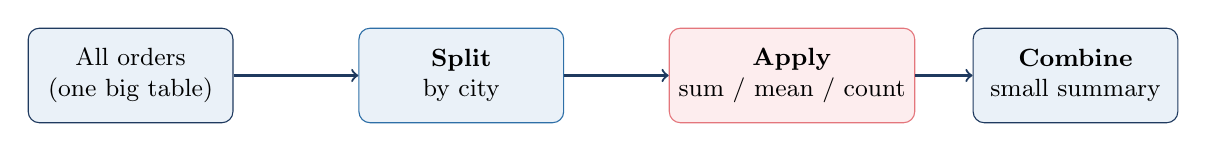
\begin{tikzpicture}[node distance=3.2cm, every node/.style={font=\small}]
    \node[draw=navy,fill=paleblue,rounded corners,minimum width=2.6cm,minimum height=1.2cm,align=center] (a) {All orders\\(one big table)};
    \node[draw=skyblue,fill=paleblue,rounded corners,right of=a,minimum width=2.6cm,minimum height=1.2cm,align=center,xshift=1cm] (b) {\textbf{Split}\\by city};
    \node[draw=coral,fill=palered,rounded corners,right of=b,minimum width=2.6cm,minimum height=1.2cm,align=center,xshift=1cm] (c) {\textbf{Apply}\\sum / mean / count};
    \node[draw=navy,fill=paleblue,rounded corners,right of=c,minimum width=2.6cm,minimum height=1.2cm,align=center,xshift=0.4cm] (d) {\textbf{Combine}\\small summary};
    \draw[->,thick,navy] (a) -- (b);
    \draw[->,thick,navy] (b) -- (c);
    \draw[->,thick,navy] (c) -- (d);
  \end{tikzpicture}
  \end{center}
  \vspace{2mm}
  \scenario{Sort a pile of receipts into one heap per city, add up each heap, and write the
  totals on a single sheet. That is exactly what \code{groupby} does.}
\end{frame}

\begin{frame}[fragile]{\texttt{groupby} basics}
\begin{lstlisting}
df.groupby("city")["total"].sum()          # revenue per city
df.groupby("city")["total"].mean()         # average order per city
df.groupby("city").size()                  # number of rows per city
df.groupby("city")["customer"].nunique()   # unique customers per city

df.groupby("city", as_index=False)["total"].sum()   # keep "city" as a normal column
\end{lstlisting}
  \begin{block}{Formula to remember}
    \code{df.groupby(WHAT TO GROUP BY)[WHICH COLUMN].WHAT TO CALCULATE()}
  \end{block}
  \scenario{``How much money did each city bring in?'' Group by city, sum the total.}
\end{frame}

\begin{frame}[fragile]{Many summaries at once: \texttt{agg}}
\begin{lstlisting}
summary = df.groupby("city").agg(
    revenue=("total", "sum"),          # new_name=(column, function)
    orders=("order_id", "count"),
    avg_order=("total", "mean"),
    best_order=("total", "max"),
)
summary.sort_values("revenue", ascending=False)
\end{lstlisting}
  \scenario{Create a one-page report for your boss: for each city show total revenue, number
  of orders, average order, and biggest order. \textbf{Named aggregation} gives clean
  column names automatically.}
\end{frame}

\begin{frame}[fragile]{Grouping by several columns}
\begin{lstlisting}
df.groupby(["city", "category"], as_index=False)["total"].sum()

# Then reshape if you like:
df.groupby(["city", "category"])["total"].sum().unstack()
\end{lstlisting}
  \scenario{``Which product category sells best \emph{in each city}?'' Group by city and
  category together. Maybe Dhaka loves keyboards, while Sylhet prefers phone cases.}
  \begin{block}{Sorted within each group}
    \code{df.sort\_values("total", ascending=False).groupby("city").head(3)} gives the top 3
    orders \textbf{per city}.
  \end{block}
\end{frame}

\begin{frame}[fragile]{\texttt{transform}: keep the original size}
\begin{lstlisting}
# agg shrinks the table (one row per group)
# transform keeps ALL rows, filling in the group's result
df["city_avg"]  = df.groupby("city")["total"].transform("mean")
df["vs_avg"]    = df["total"] - df["city_avg"]
df["pct_of_city"] = df["total"] / df.groupby("city")["total"].transform("sum") * 100
\end{lstlisting}
  \scenario{``Is this order bigger than a typical order \emph{in the same city}?'' You need
  the city average next to each order, so you use \code{transform}.}
  \begin{block}{agg or transform?}
    Want a \textbf{summary table}? \code{agg}. Want a \textbf{new column} on the original
    table? \code{transform}.
  \end{block}
\end{frame}

\begin{frame}[fragile]{Filtering whole groups}
\begin{lstlisting}
# Keep only customers who placed at least 3 orders
loyal = df.groupby("customer").filter(lambda g: len(g) >= 3)

# Same idea, often faster:
counts = df.groupby("customer")["order_id"].transform("count")
loyal = df[counts >= 3]
\end{lstlisting}
  \scenario{Send a thank-you coupon only to customers with 3 or more orders. You filter
  \emph{groups}, not individual rows.}
\end{frame}

\begin{frame}[fragile]{\texttt{pivot\_table}: Excel's pivot table}
\begin{lstlisting}
pd.pivot_table(
    df,
    index="city",              # rows
    columns="category",        # columns
    values="total",            # what to calculate
    aggfunc="sum",             # how
    fill_value=0,              # show 0 instead of NaN
    margins=True,              # add "All" totals
)
\end{lstlisting}
  \scenario{A manager wants a grid: cities down the side, categories across the top, revenue
  inside each cell. This is the classic pivot report.}
  \begin{block}{groupby or pivot\_table?}
    Same maths. \code{groupby} is flexible; \code{pivot\_table} gives a \textbf{wide grid}
    that is easier to read.
  \end{block}
\end{frame}

\begin{frame}[fragile]{\texttt{crosstab}: count combinations}
\begin{lstlisting}
pd.crosstab(df["city"], df["category"])                         # counts
pd.crosstab(df["city"], df["category"], normalize="index")      # row percentages
pd.crosstab(df["city"], df["status"], margins=True)             # with totals
\end{lstlisting}
  \scenario{``What share of orders in each city were returned?'' A crosstab of city versus
  status, normalized by rows, shows the percentages instantly.}
\end{frame}

\begin{frame}{Summarizing: which tool should I use?}
  \small
  \renewcommand{\arraystretch}{1.25}
  \begin{center}
  \begin{tabular}{p{5.5cm}p{5.5cm}}
    \toprule
    \textbf{Question} & \textbf{Tool}\\
    \midrule
    One number for the whole column & \code{df["x"].sum() / mean()}\\
    Number per category & \code{groupby("cat")["x"].sum()}\\
    Several numbers per category & \code{groupby().agg(name=(col, fn))}\\
    Group result next to every row & \code{groupby().transform()}\\
    Keep only big/small groups & \code{groupby().filter()}\\
    Grid of category $\times$ category & \code{pivot\_table}\\
    Count of combinations & \code{crosstab} or \code{value\_counts}\\
    \bottomrule
  \end{tabular}
  \end{center}
\end{frame}

% ============================================================
\section{Combining tables}

\begin{frame}[fragile]{\texttt{concat}: stack tables}
\begin{lstlisting}
jan = pd.read_csv("orders_jan.csv")
feb = pd.read_csv("orders_feb.csv")
mar = pd.read_csv("orders_mar.csv")

all_orders = pd.concat([jan, feb, mar], ignore_index=True)   # stack on top

# Remember where each row came from
all_orders = pd.concat({"Jan": jan, "Feb": feb, "Mar": mar}, names=["month"])

# Side by side (columns) when rows line up
pd.concat([df_a, df_b], axis=1)
\end{lstlisting}
  \scenario{You get one file per month. \code{concat} glues all 12 into a single yearly table
  (same columns, more rows).}
\end{frame}

\begin{frame}[fragile]{\texttt{merge}: like a SQL JOIN or Excel VLOOKUP}
\begin{lstlisting}
orders    = pd.DataFrame({"order_id": [1, 2, 3], "customer_id": [10, 11, 10]})
customers = pd.DataFrame({"customer_id": [10, 11, 12], "name": ["Rafi", "Mim", "Sara"]})

pd.merge(orders, customers, on="customer_id", how="left")
\end{lstlisting}
  \scenario{The orders table only has a customer ID. The customers table has names and
  cities. \code{merge} attaches the names to each order using the shared ID,
  just like a lookup in Excel.}
  \begin{block}{Different key names?}
    \code{pd.merge(a, b, left\_on="cust\_id", right\_on="id")}
  \end{block}
\end{frame}

\begin{frame}{Merge types: \texttt{how=}}
  \renewcommand{\arraystretch}{1.3}
  \begin{center}
  \small
  \begin{tabular}{p{1.8cm}p{4.5cm}p{4.8cm}}
    \toprule
    \textbf{how} & \textbf{Keeps} & \textbf{Use when}\\
    \midrule
    \code{inner} & Only matches in BOTH & You only want complete info\\
    \code{left} & Everything from the left, matches from right & Keep all orders, add customer info
      (\textbf{most common})\\
    \code{right} & Everything from the right & Rarely used (swap tables and use left)\\
    \code{outer} & Everything from both & Find what is missing on either side\\
    \bottomrule
  \end{tabular}
  \end{center}
  \scenario{\code{left}: ``Show all orders, even if the customer isn't registered.''
  \code{inner}: ``Show only orders from registered customers.''}
\end{frame}

\begin{frame}[fragile]{Merge safely}
\begin{lstlisting}
pd.merge(
    orders, customers, on="customer_id", how="left",
    validate="m:1",        # many orders -> one customer. Error if customers has duplicates
    indicator=True,        # adds "_merge" column: both / left_only / right_only
    suffixes=("_order", "_cust"),   # names for clashing column names
)
\end{lstlisting}
  \begin{alertblock}{Why validate?}
    If the customers table accidentally contains duplicate IDs, a merge silently
    \textbf{multiplies} your rows and inflates revenue. \code{validate} catches it.
  \end{alertblock}
  \begin{block}{Check after every merge}
    Compare \code{len()} before and after. For a \code{left} merge with \code{m:1}, the row
    count must stay the same.
  \end{block}
\end{frame}

\begin{frame}[fragile]{\texttt{join}: merge on the index}
\begin{lstlisting}
customers = customers.set_index("customer_id")
orders.join(customers, on="customer_id")        # use orders' column, customers' index
\end{lstlisting}
  \begin{block}{merge or join or concat?}
    \textbf{concat}: same columns, stack more rows (or put tables side by side).\\
    \textbf{merge}: match rows using a shared column (most flexible).\\
    \textbf{join}: shortcut for merging on the index.
  \end{block}
\end{frame}

% ============================================================
\section{Dates and time series}

\begin{frame}[fragile]{Working with dates}
\begin{lstlisting}
df["date"] = pd.to_datetime(df["date"])       # text -> datetime
df["year"]     = df["date"].dt.year
df["month"]    = df["date"].dt.month
df["weekday"]  = df["date"].dt.day_name()     # "Monday", "Tuesday"...
df["quarter"]  = df["date"].dt.quarter
df["is_weekend"] = df["date"].dt.dayofweek >= 5

(pd.Timestamp("2026-12-31") - df["date"]).dt.days    # days until year end
\end{lstlisting}
  \scenario{``Do we sell more on weekends?'' Create a weekday column and group by it.}
  \begin{block}{Tip}
    Use \code{pd.to\_datetime(df["d"], format="\%d/\%m/\%Y")} if dates are written day-first.
  \end{block}
\end{frame}

\begin{frame}[fragile]{Date index and slicing}
\begin{lstlisting}
ts = df.set_index("date").sort_index()

ts.loc["2026-03"]                     # everything in March 2026
ts.loc["2026-01-15":"2026-02-15"]     # a date range
ts["total"].loc["2026"]               # whole year
\end{lstlisting}
  \scenario{Compare ``this week'' with ``last week'' by slicing date ranges with
  plain text. No complicated conditions.}
\end{frame}

\begin{frame}[fragile]{\texttt{resample}: change the time step}
\begin{lstlisting}
ts["total"].resample("D").sum()     # daily sales
ts["total"].resample("W").sum()     # weekly sales
ts["total"].resample("ME").sum()    # monthly sales ("ME" = month end)
ts["total"].resample("QE").mean()   # quarterly average

monthly = ts["total"].resample("ME").sum()
monthly.plot(kind="line", title="Monthly revenue")
\end{lstlisting}
  \scenario{Orders arrive every minute. Your boss wants one number per month to see the trend.
  \code{resample("ME").sum()} does it in one line.}
  \begin{block}{resample vs groupby}
    \code{resample} = group by \textbf{time buckets} (needs a date index). \code{groupby} =
    group by anything.
  \end{block}
\end{frame}

\begin{frame}[fragile]{Rolling windows: smooth the noise}
\begin{lstlisting}
daily = ts["total"].resample("D").sum()

daily.rolling(7).mean()              # 7-day moving average
daily.rolling(7, min_periods=1).sum()   # last 7 days total
daily.expanding().sum()              # running total since day 1
daily.ewm(span=7).mean()             # recent days count more
\end{lstlisting}
  \scenario{Daily sales jump up and down. The 7-day moving average smooths the zigzag so you
  can see if the business is really growing, just like a stock chart.}
\end{frame}

\begin{frame}[fragile]{Compare with the past: \texttt{shift}, \texttt{diff}, \texttt{pct\_change}}
\begin{lstlisting}
monthly = ts["total"].resample("ME").sum()

monthly.shift(1)          # last month's value on this month's row
monthly.diff()            # this month minus last month
monthly.pct_change() * 100   # growth in percent
monthly.pct_change(12)    # compared with same month last year
\end{lstlisting}
  \scenario{``Did sales grow in March compared to February?'' \code{pct\_change} gives the
  answer for every month at once.}
\end{frame}

% ============================================================
\section{Advanced techniques}

\begin{frame}[fragile]{MultiIndex: more than one row label}
\begin{lstlisting}
g = df.groupby(["city", "category"])["total"].sum()   # two-level index

g.loc["Dhaka"]                    # all categories in Dhaka
g.loc[("Dhaka", "Keyboard")]      # one exact value
g.xs("Keyboard", level="category")  # Keyboard in every city
g.reset_index()                   # flatten back to a normal table
\end{lstlisting}
  \scenario{Think of folders inside folders: City $\rightarrow$ Category $\rightarrow$ number.
  Beginners can use \code{reset\_index()} to avoid it, and advanced users use it for
  powerful slicing.}
\end{frame}

\begin{frame}[fragile]{\texttt{melt}: wide table to long table}
\begin{lstlisting}
scores = pd.DataFrame({
    "student": ["Rafi", "Mim"],
    "math": [90, 85], "science": [80, 95], "english": [70, 88],
})

long = scores.melt(id_vars="student", var_name="subject", value_name="score")
#   student  subject  score
#   Rafi     math     90
#   Mim      math     85 ...
\end{lstlisting}
  \scenario{Your exam sheet has one column per subject (wide). To make a chart or
  \code{groupby("subject")}, you need one row per score (long). \code{melt} converts it.}
\end{frame}

\begin{frame}[fragile]{\texttt{pivot}, \texttt{stack}, \texttt{unstack}: reshape back}
\begin{lstlisting}
long.pivot(index="student", columns="subject", values="score")   # long -> wide

s = df.groupby(["city", "category"])["total"].sum()
s.unstack()          # move the inner index level to columns
s.unstack().stack()  # and back again
\end{lstlisting}
  \begin{block}{Remember}
    \code{melt}: wide $\rightarrow$ long. \code{pivot}: long $\rightarrow$ wide (no maths).
    \code{pivot\_table}: long $\rightarrow$ wide \textbf{with aggregation}.
  \end{block}
\end{frame}

\begin{frame}[fragile]{Categorical data}
\begin{lstlisting}
df["size"] = pd.Categorical(
    df["size"], categories=["Small", "Medium", "Large"], ordered=True
)
df.sort_values("size")             # sorts Small < Medium < Large (not A-Z!)
df[df["size"] >= "Medium"]         # ordered comparison works

df["city"] = df["city"].astype("category")   # saves memory for repeated text
\end{lstlisting}
  \scenario{T-shirt sizes sorted alphabetically give Large, Medium, Small, which is wrong.
  An \textbf{ordered category} sorts them logically.}
\end{frame}

\begin{frame}[fragile]{Group-wise running totals and ranks}
\begin{lstlisting}
df = df.sort_values(["customer", "date"])

df["running_total"] = df.groupby("customer")["total"].cumsum()
df["order_number"]  = df.groupby("customer").cumcount() + 1
df["rank_in_city"]  = df.groupby("city")["total"].rank(ascending=False)
df["prev_order"]    = df.groupby("customer")["total"].shift(1)
\end{lstlisting}
  \scenario{For each customer, show their 1st, 2nd, 3rd order, how much they have spent so
  far, and whether the new order is bigger than the previous one. Perfect for finding
  customers who spend more over time.}
\end{frame}

\begin{frame}[fragile]{Lists inside cells: \texttt{explode}}
\begin{lstlisting}
posts = pd.DataFrame({
    "post": ["A", "B"],
    "tags": [["python", "pandas"], ["python", "excel", "tips"]],
})
posts.explode("tags")                  # one row per tag

# Text with commas -> list -> rows
df["tags"].str.split(",").explode().str.strip().value_counts()
\end{lstlisting}
  \scenario{Each blog post has several tags. To count ``which tag is used most?'' first
  explode so each tag has its own row, then \code{value\_counts}.}
\end{frame}

\begin{frame}[fragile]{Method chaining and \texttt{pipe}}
\begin{lstlisting}
result = (
    pd.read_csv("sunnymart_orders.csv", parse_dates=["date"])
      .dropna(subset=["price"])
      .drop_duplicates("order_id")
      .assign(total=pd.col("qty") * pd.col("price"))
      .query("total > 0")
      .groupby("city", as_index=False)["total"].sum()
      .sort_values("total", ascending=False)
      .head(5)
)
\end{lstlisting}
  \begin{itemize}
    \item Reads top to bottom like a recipe; no half-finished variables.
    \item Use \code{.pipe(my\_function)} to put your own function inside a chain.
  \end{itemize}
\end{frame}

\begin{frame}[fragile]{Make your code fast}
\begin{lstlisting}
# 1. Load less
df = pd.read_csv("big.csv", usecols=["city", "total"], dtype={"city": "category"})

# 2. Read a huge file in pieces
for chunk in pd.read_csv("huge.csv", chunksize=100_000):
    part = chunk.groupby("city")["total"].sum()      # process, then combine

# 3. Check memory
df.info(memory_usage="deep")

# 4. Use Parquet instead of CSV
df.to_parquet("big.parquet");  pd.read_parquet("big.parquet")
\end{lstlisting}
  \begin{alertblock}{Speed tips}
    Avoid \code{iterrows()} and \code{apply(axis=1)}. Use vectorized maths, \code{category}
    for repeated text, smaller number types, and Parquet files.
  \end{alertblock}
\end{frame}

\begin{frame}{pandas 3.0: what changed? (from the official release notes)}
  \begin{columns}[T]
    \column{0.48\textwidth}
    \begin{block}{Copy-on-Write is default}
      Anything you get from filtering or selecting \textbf{behaves as a copy}. Changing it
      never changes the original by accident. No more \code{SettingWithCopyWarning}.
    \end{block}
    \begin{block}{Dedicated \code{str} dtype}
      Text columns now have dtype \code{str} instead of \code{object}. Faster and clearer
      (PyArrow-backed when installed).
    \end{block}
    \column{0.48\textwidth}
    \begin{block}{\code{pd.col()}}
      Refer to a column by name inside \code{assign}, without repeating the DataFrame
      name or writing a lambda.
    \end{block}
    \begin{alertblock}{What to do}
      Update to Python 3.11+, and always modify with \code{df.loc[mask, "col"] = value}.
      Don't check for \code{dtype == object} to find text columns; use
      \code{df.select\_dtypes("string")} or \code{pd.api.types.is\_string\_dtype}.
    \end{alertblock}
  \end{columns}
\end{frame}

\begin{frame}[fragile]{Quick charts with pandas}
\begin{lstlisting}
import matplotlib.pyplot as plt             # pip install matplotlib

by_city = df.groupby("city")["total"].sum().sort_values()
by_city.plot(kind="barh", title="Revenue by city")      # horizontal bars

df["total"].plot(kind="hist", bins=20)                   # distribution
monthly.plot(kind="line", marker="o")                    # trend over time
df.plot(kind="scatter", x="price", y="qty")              # relationship
plt.show()
\end{lstlisting}
  \begin{block}{Which chart?}
    \textbf{Bar}: compare categories. \textbf{Line}: change over time. \textbf{Hist}: how
    values are spread. \textbf{Scatter}: do two numbers move together?
  \end{block}
\end{frame}

\begin{frame}[fragile]{Display options and styling}
\begin{lstlisting}
pd.set_option("display.max_columns", 50)         # show all columns
pd.set_option("display.float_format", "{:,.2f}".format)   # 12,345.60
pd.reset_option("all")

# Colour a table in Jupyter
summary.style.background_gradient(cmap="Blues").format("{:,.0f}")
\end{lstlisting}
  \scenario{Present results to your teacher or boss. A coloured, nicely formatted table
  looks much more professional than raw numbers.}
\end{frame}

% ============================================================
\section{Mini project and wrap-up}

\begin{frame}[fragile]{Mini project: Sunny Mart report (steps 1--2)}
\begin{lstlisting}
import pandas as pd

# 1) LOAD
df = pd.read_csv("sunnymart_orders.csv", parse_dates=["date"])
df.info()

# 2) CLEAN
df.columns = df.columns.str.strip().str.lower()
df["city"] = df["city"].str.strip().str.title().fillna("Unknown")
df["price"] = pd.to_numeric(df["price"], errors="coerce")
df = df.dropna(subset=["price"]).drop_duplicates("order_id")
df = df[(df["qty"] > 0) & (df["price"] > 0)]
\end{lstlisting}
\end{frame}

\begin{frame}[fragile]{Mini project: Sunny Mart report (steps 3--5)}
\begin{lstlisting}
# 3) TRANSFORM
df["total"] = df["qty"] * df["price"]
df["month"] = df["date"].dt.to_period("M")

# 4) ANALYSE
top_cities = df.groupby("city")["total"].sum().nlargest(5)
best_items = df.groupby("product")["total"].sum().nlargest(5)
monthly    = df.groupby("month")["total"].sum()
growth     = monthly.pct_change() * 100
vip        = df.groupby("customer")["total"].sum().nlargest(10)

# 5) SHARE
top_cities.plot(kind="bar", title="Top 5 cities")
top_cities.to_csv("top_cities.csv")
\end{lstlisting}
  \alert{Answers for the boss:} best cities, best products, monthly growth, and top customers.
\end{frame}

\begin{frame}{Common errors and how to fix them}
  \small
  \renewcommand{\arraystretch}{1.25}
  \begin{tabular}{p{4.4cm}p{6.6cm}}
    \toprule
    \textbf{Error / problem} & \textbf{Fix}\\
    \midrule
    \code{KeyError: 'City'} & Check spelling and capitals with \code{df.columns}\\
    \code{truth value of a Series is ambiguous} & Use \code{\&}, \code{|}, and parentheses\\
    Values didn't change after assignment & Use \code{df.loc[mask, "col"] = ...}, no chaining\\
    \code{ValueError: could not convert string} & \code{pd.to\_numeric(errors="coerce")}\\
    Row count doubled after merge & Duplicate keys: use \code{validate="m:1"}\\
    Sum looks wrong & Check for duplicates, NaN, and wrong dtypes\\
    Strange extra column \code{Unnamed: 0} & Save with \code{to\_csv(index=False)}\\
    \bottomrule
  \end{tabular}
\end{frame}

\begin{frame}{Master cheat sheet: when to use what}
  \scriptsize
  \renewcommand{\arraystretch}{1.15}
  \begin{tabular}{p{3.4cm}p{4.0cm}p{4.2cm}}
    \toprule
    \textbf{Goal} & \textbf{Method} & \textbf{Scenario}\\
    \midrule
    Load data & \code{read\_csv, read\_excel} & Boss sends a file\\
    Inspect & \code{head, info, describe} & First look at new data\\
    Filter rows & \code{df[mask], query} & Orders above \$20\\
    Pick cells & \code{loc, iloc} & Row by name or position\\
    Missing & \code{isna, dropna, fillna} & Blank city boxes\\
    Duplicates & \code{drop\_duplicates} & Double-sent payments\\
    Types & \code{astype, to\_datetime} & Text prices, text dates\\
    Text & \code{.str.*} & Messy names\\
    If-else & \code{np.where, np.select} & Free delivery tiers\\
    Bins & \code{cut, qcut} & Age groups, top 25\%\\
    Summaries & \code{groupby + agg} & Revenue per city\\
    Excel-style grid & \code{pivot\_table} & City $\times$ category\\
    Stack files & \code{concat} & 12 monthly files\\
    Lookup & \code{merge} & Add names to orders\\
    Trends & \code{resample, rolling} & Monthly growth\\
    Reshape & \code{melt, pivot} & Wide exam sheet to long\\
    \bottomrule
  \end{tabular}
\end{frame}

\begin{frame}{Practice challenges}
  Download any CSV (try Kaggle or your school's data) and solve:
  \begin{enumerate}
    \item Load it, check \code{info()}, and count missing values per column.
    \item Clean text columns and convert date columns to datetime.
    \item Find the top 5 categories by total value.
    \item Create a new column using \code{np.select} with three tiers.
    \item Make a pivot table and a line chart by month.
    \item Merge it with a second small table (a lookup list).
    \item Rewrite your whole analysis as one \alert{method chain}.
  \end{enumerate}
\end{frame}

\begin{frame}{Where to learn next (official resources)}
  \begin{itemize}
    \item \textbf{pandas documentation:} \texttt{pandas.pydata.org/docs}
    \item \textbf{10 minutes to pandas:} the official quick start
    \item \textbf{User Guide:} deep explanations of every topic
    \item \textbf{API Reference:} every function with examples
    \item \textbf{What's new in 3.0:} \texttt{pandas.pydata.org/docs/whatsnew/v3.0.0.html}
    \item \textbf{Next skills:} NumPy, Matplotlib/Seaborn, SQL, then scikit-learn
  \end{itemize}
  \vspace{3mm}
  \begin{block}{Final advice}
    Don't memorize everything. Learn the \emph{ideas} (select, clean, transform, group,
    combine) and keep the docs open while you code. Professionals do exactly that.
  \end{block}
\end{frame}

\begin{frame}[plain]
  \centering
  \vfill
  {\color{navy}\Huge\bfseries Thank you!}\\[4mm]
  {\color{coral}\Large Now open a notebook and try the code.}\\[6mm]
  {\color{ink}\large Happy data exploring with pandas}
  \vfill
\end{frame}

\end{document}
